\documentclass[11pt, A4paper,norsk]{article}
\usepackage[utf8]{inputenc}
\usepackage[T1]{fontenc}
\usepackage{babel}
\usepackage{amsmath}
\usepackage{amsfonts}
\usepackage{amsthm}
\usepackage{amssymb}
\usepackage[colorlinks]{hyperref}
\usepackage{listings}
\usepackage{color}
\usepackage{hyperref}
\usepackage{graphicx}
\usepackage{cite}
\usepackage{textcomp}
\usepackage{float}

\definecolor{dkgreen}{rgb}{0,0.6,0}
\definecolor{gray}{rgb}{0.5,0.5,0.5}
\definecolor{daynineyellow}{rgb}{1.0,0.655,0.102}
\definecolor{url}{rgb}{0.1,0.1,0.4}

\lstset{frame=tb,
	language=Python,
	aboveskip=3mm,
	belowskip=3mm,
	showstringspaces=false,
	columns=flexible,
	basicstyle={\small\ttfamily},
	numbers=none,
	numberstyle=\tiny\color{gray},
	keywordstyle=\color{blue},
	commentstyle=\color{daynineyellow},
	stringstyle=\color{dkgreen},
	breaklines=true,
	breakatwhitespace=true,
	tabsize=3
}

\lstset{inputpath="C:/Users/Torstein/Documents/UiO/Fys2130/Python programmer"}
\graphicspath{{C:/Users/Torstein/Documents/UiO/Fys2130/"Python programmer"/}}
\hypersetup{colorlinks, urlcolor=url}

\author{Torstein Solheim Ølberg}
\title{Svar på Oblig nr. 3 i Fys2130}



%\lstinputlisting{Filnavn! type kodefil}
%\includegraphics[width=12.6cm,height=9cm]{Filnavn! type png}



\begin{document}
\maketitle
	\begin{center}
\Large \textbf{Oppgaver}
	\end{center}









		\paragraph{5)}
			\subparagraph{2.}
				\begin{flushleft}
Hvis vi ikke hadde dette filteret så kunne cden antatt at målingnene hørte til andre bølger enn det vi har spilt inn på og vi kunne fått helt annen lyd. Dette komemr av at vi er nødt til å måle minst to ganger per bølgelengde til bølgen for å være sikker på at vi får riktig bølge.
				\end{flushleft}









		\paragraph{14)}
			\subparagraph{1.}
				\begin{flushleft}
Den viktigste forskjellen på Fourieranalyse og waveletanalyse er at wavelet analyse tar hensyn til at et signal kan endre seg med tiden, mens Fourieranalyse er stasjonært i tiden og derfor ubrukelig hvis signalet endrer seg mye.
				\end{flushleft}









			\subparagraph{2.}
				\begin{flushleft}
Fouriertransformasjon gir et ganske ubrukelig resultat hvis bølgen varierer mye fra en tidsperiode til den neste.
				\end{flushleft}
			









			\subparagraph{3.}
				\begin{flushleft}
Wavelet har ulempen at du er nødt til å velge hele tidsintervallet du ønske å analysere over på forhånd istedenfor å kunne holde på konstant i ubestemt tid, slik som ved en Fouriertransformasjon.
				\end{flushleft}










			\subparagraph{5.}
				\begin{flushleft}
Det som menes med at Wavelet har et randproblem er at når du analyserer et signal med en wavelet vil bare halve waveletten bli brukt i starten eller i slutten av signalet. Dette gjør at de verdiene vi får fra å analysere verdiene i ytterkantene blir mye mindre enn alle andre steder. Antar at med randverdisonen så menes den sonen der det er et randproblem. Da blir ranverdisonen halvparten av bredden til waveletten din
				\end{flushleft}









		\paragraph{5)}
			\subparagraph{8.}
				\begin{flushleft}
Finner Fouriertransformasjon for et diskret signal på side $98$ i læreboka.
				\end{flushleft}
				\begin{gather*}
X_k = \frac{1}{N} \sum_{n = 0}^{N - 1} x_n e^{-i\frac{2 \pi}{N} kn} \\
X_0 = \frac{1}{N} \sum_{n = 0}^{N - 1} x_n e^{0} \\
X_0 = \frac{x_0 + x_1 + x_2 + \dots + x_{N - 1}}{N} \\
\text{Dette er gjennomsnittet av utgangssignalet.}
				\end{gather*}
				\begin{flushleft}
Lager en FT funksjon og tester for et selvlaget signal jeg vet gjennomsnittsverdien til. Det som printes er først den utregnete verdien ved hjelp av Fouriertransformansjon for $k = 0$ og den andre verdien som printes er bare summen av verdiene i signalet delt på antall verdier. Begge disse blir korekte og lik $2$.
				\end{flushleft}
\lstinputlisting{Oblig3_5_8.py}







			\subparagraph{9.}
\lstinputlisting{Oblig3_5_9.py}
				\begin{flushleft}
Fikk disse plottene
				\end{flushleft}
				\begin{figure}[H]
\caption{Plott for $100 Hz$ som frekvens}
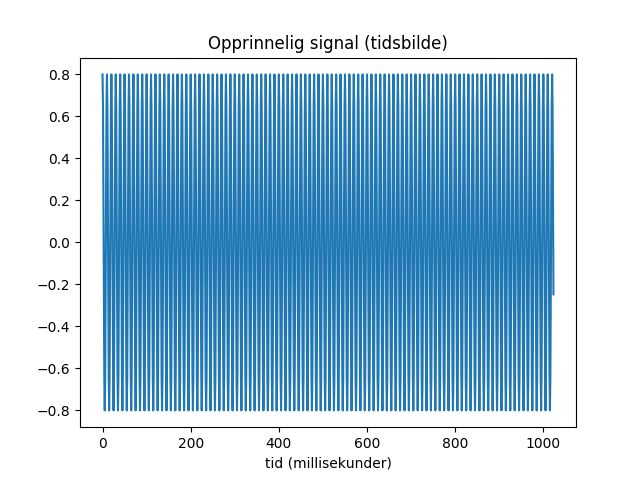
\includegraphics[width=12.6cm,height=8cm]{3Figur_00.png} \\
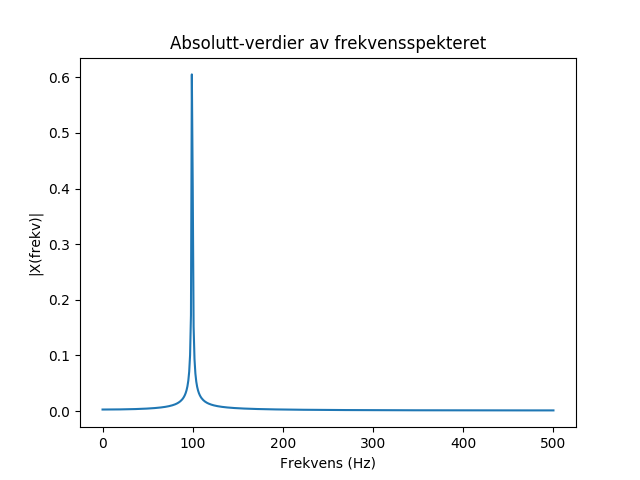
\includegraphics[width=12.6cm,height=8cm]{3Figur_01.png} \\
				\end{figure}
				\begin{figure}[H]
\caption{Plott for $200 Hz$ som frekvens}
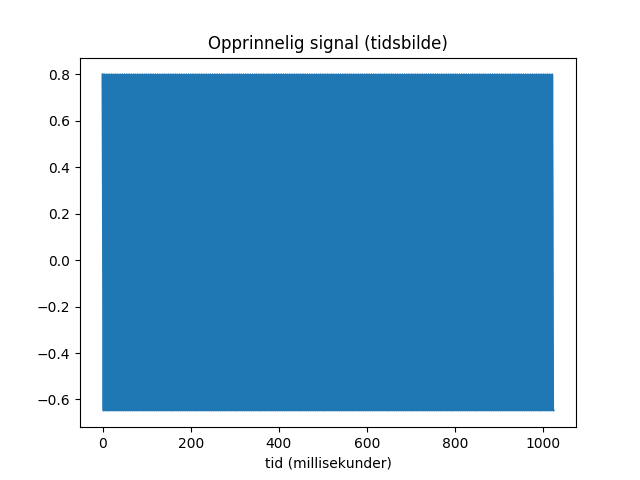
\includegraphics[width=12.6cm,height=8cm]{3Figur_02.png} \\
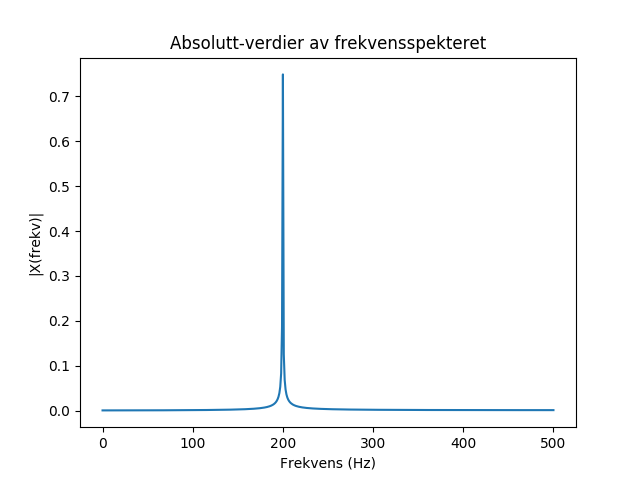
\includegraphics[width=12.6cm,height=8cm]{3Figur_03.png} \\
				\end{figure}
				\begin{figure}[H]
\caption{Plott for $400 Hz$ som frekvens}
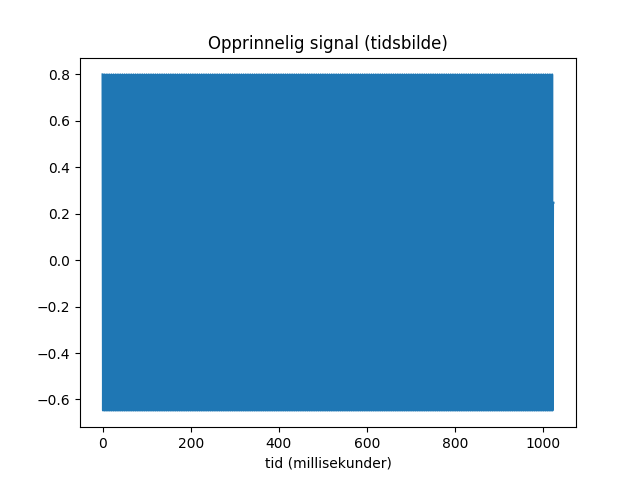
\includegraphics[width=12.6cm,height=8cm]{3Figur_04.png} \\
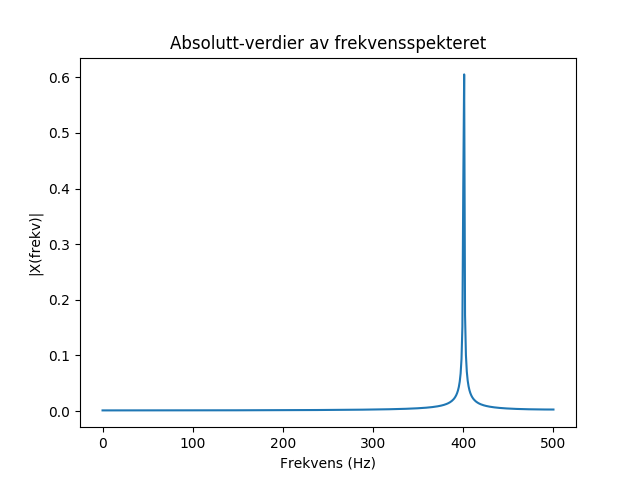
\includegraphics[width=12.6cm,height=8cm]{3Figur_05.png} \\
				\end{figure}
				\begin{figure}[H]
\caption{Plott for $700 Hz$ som frekvens}
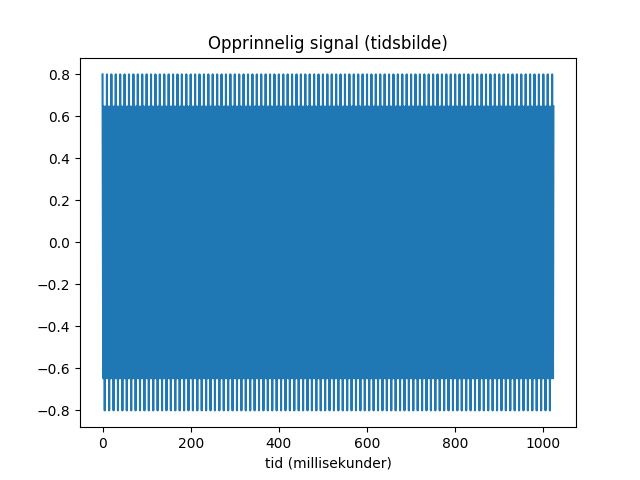
\includegraphics[width=12.6cm,height=8cm]{3Figur_06.png} \\
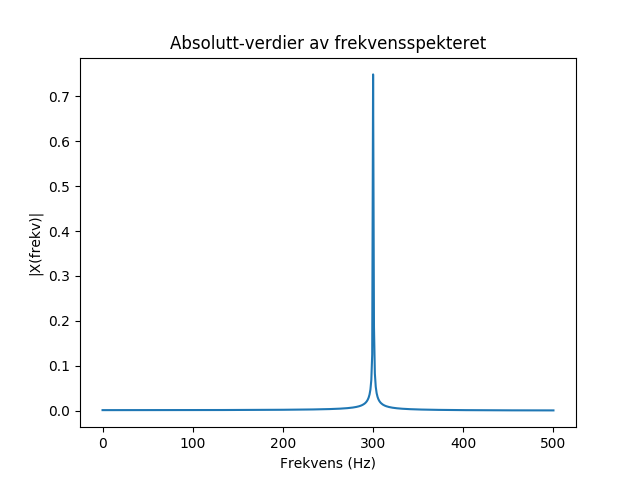
\includegraphics[width=12.6cm,height=8cm]{3Figur_07.png} \\
				\end{figure}
				\begin{figure}[H]
\caption{Plott for $950 Hz$ som frekvens}
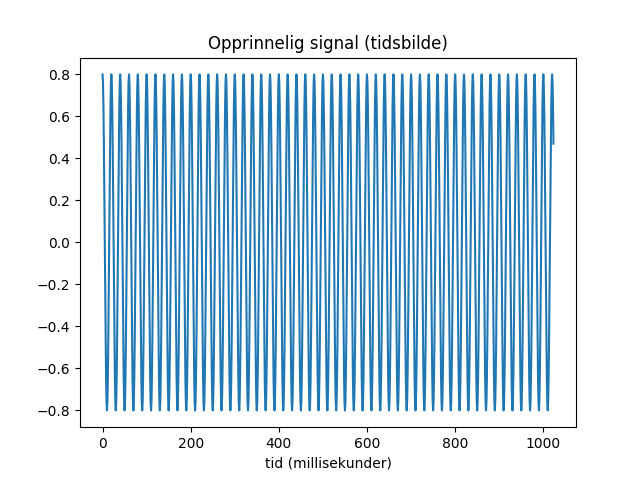
\includegraphics[width=12.6cm,height=8cm]{3Figur_09.png} \\
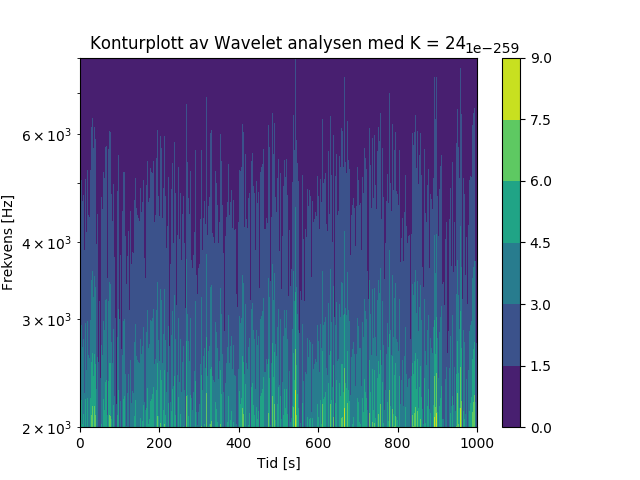
\includegraphics[width=12.6cm,height=8cm]{3Figur_10.png} \\
				\end{figure}
				\begin{figure}[H]
\caption{Plott for $1300 Hz$ som frekvens}
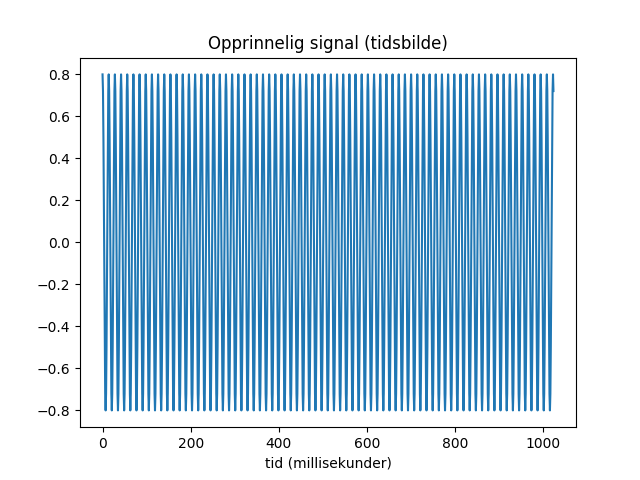
\includegraphics[width=12.6cm,height=8cm]{3Figur_12.png} \\
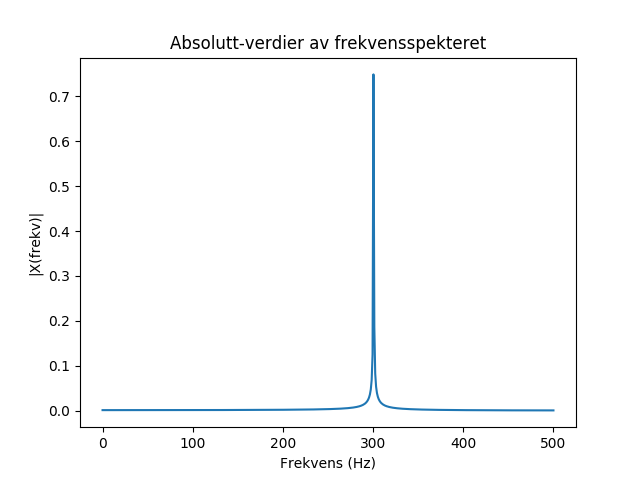
\includegraphics[width=12.6cm,height=8cm]{3Figur_13.png}
				\end{figure}
				\begin{flushleft}
Ser at toppene i frekvensbildet kommer, enten på de plassene som tilsvarer den faktiske frekvensen til signalet, eller speilet om halvparten av samplingsfrekvensen. Unntaket er når frekvensen til signalet passerer samplingsfrekvensen, da blir det en like langt fra null som frekvensen til signalet er fra null, men positiv.
				\end{flushleft}








			\subparagraph{11.}
				\begin{flushleft}
Brukte Fouriertransformasjon til å lage et frekvensbilde. Det ser ut som gjennomsnittet av amplitudene som kommer hvert tiende år er ganske lik som amplituden til frekvensbildet ganget med $10$, 
				\end{flushleft}
				\begin{figure}[H]
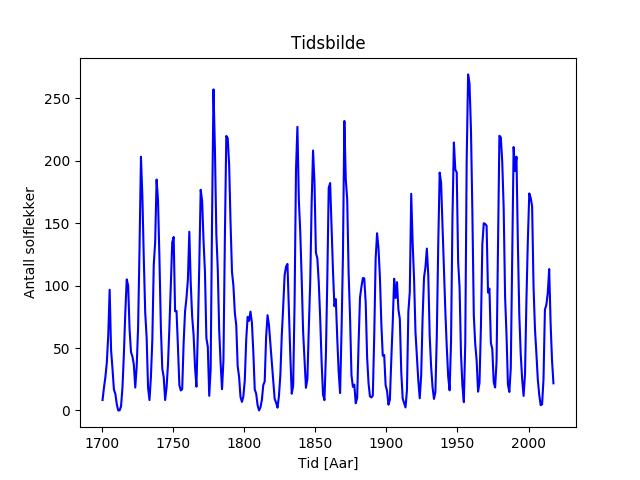
\includegraphics[width=12.6cm,height=8.0cm]{3Figur_15.png} \\
\caption{Plott av antall solflekker per år. Data hentet fra \url{http://www.sidc.be/silso/DATA/SN_y_tot_V2.0.txt}}
				\end{figure}
				\begin{figure}[H]
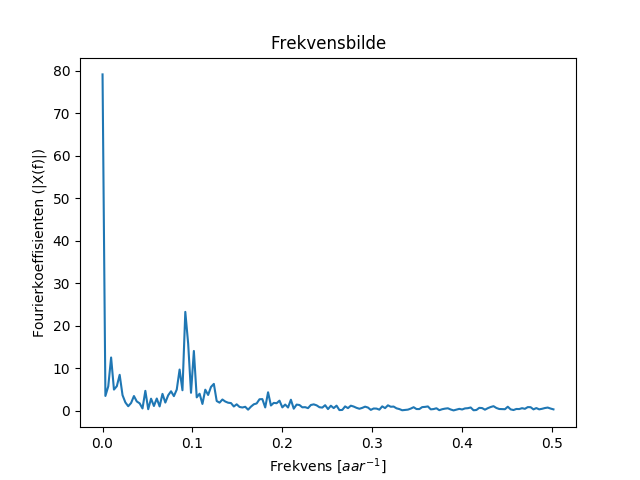
\includegraphics[width=12.6cm,height=8.0cm]{3Figur_16.png} \\
\caption{Plott av Fouriertransformasjonen av dataet fra plottet over}
				\end{figure}
\lstinputlisting{Oblig3_5_11.py}









			\subparagraph{14.}
				\begin{flushleft}
Lagde et progam som lagde en enkel harmonisk sinus bølge med frekvens $13$ over en periode på $1$ sek. Valgte amplitude $2$ og samplingsfrekvensen lik $512$, og kjørte transformasjonen. Da fikk jeg som jeg forventet et plott av en sinusbølge og ett plott av et frekvensbilde med enn stor topp ved frekvens lik $13$.
				\end{flushleft}
				\begin{figure}[H]
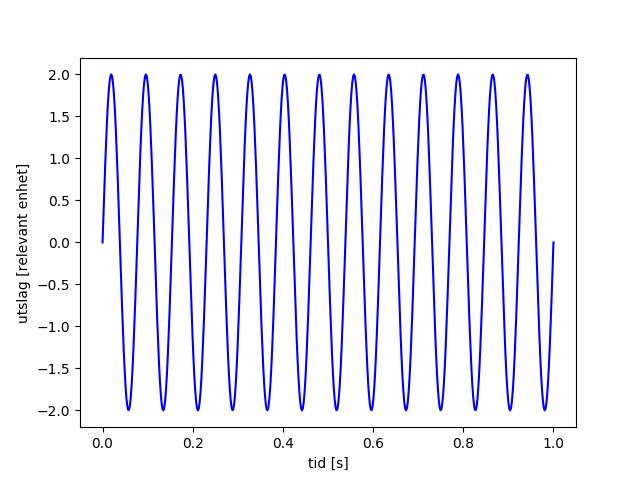
\includegraphics[width=12.6cm,height=9cm]{3Figur_17.png} \\
\caption{Sinusbølge med amplitude $2$ og frekvens $13$}
				\end{figure}
				\begin{figure}[H]
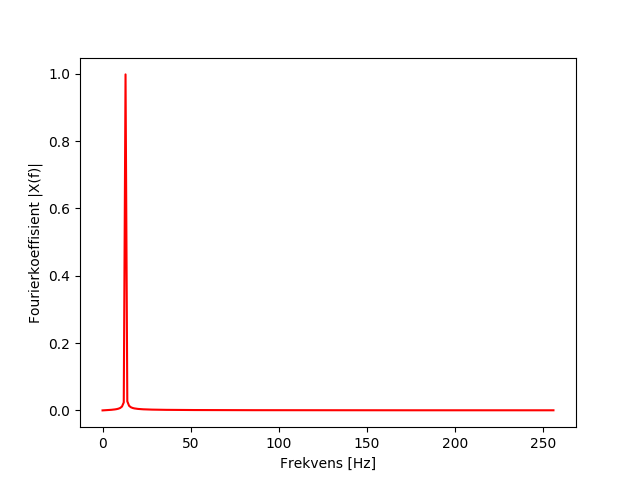
\includegraphics[width=12.6cm,height=9cm]{3Figur_18.png} \\
\caption{Fouriertransformasjon av sinusbølgen over}
				\end{figure}
\lstinputlisting{Oblig3_5_14.py}










			\subparagraph{15.}
				\begin{flushleft}
Kopierte programmet over, men endret frekvensen fra $13$ til $13.2$.
Da får jeg en sinusbølge som så vidt begynner på en ekstra periode. Denne gangen blir frekvensbildet fra den Fouriertransformerte helt likt som forrige gang, bare at den ene toppen som kommer opp er litt bredere. 
				\end{flushleft}
				\begin{figure}[H]
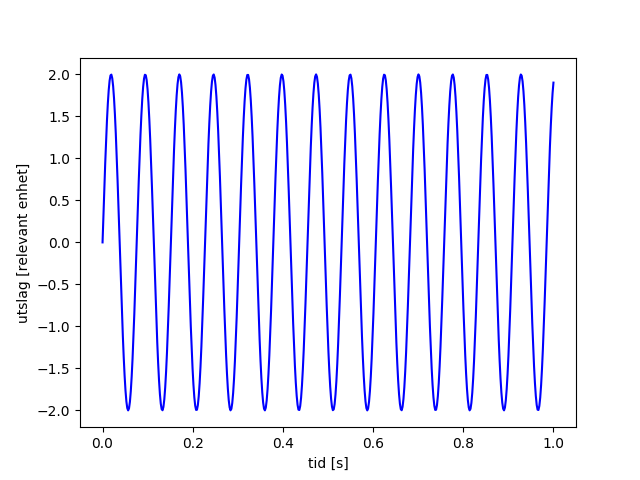
\includegraphics[width=12.6cm,height=9cm]{3Figur_19.png} \\
\caption{Sinusbølge med amplitude $2$ og frekvens $13.2$}
				\end{figure}
				\begin{figure}[H]
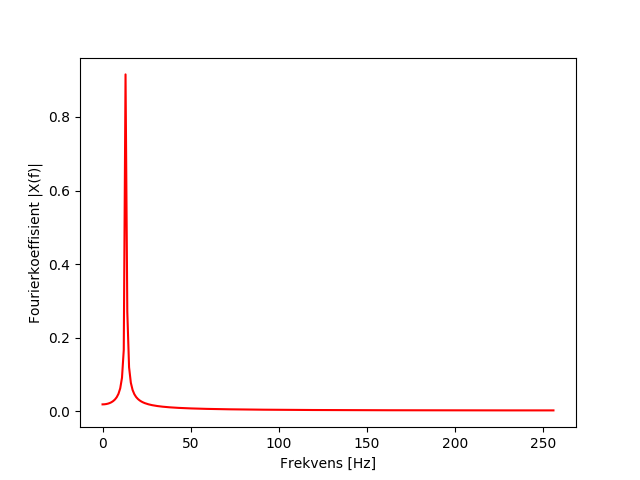
\includegraphics[width=12.6cm,height=9cm]{3Figur_20.png} \\
\caption{Fouriertransformasjon av sinusbølgen over}
				\end{figure}
\lstinputlisting{Oblig3_5_15.py}









			\subparagraph{16.}
				\begin{flushleft}
Modifiserte programmet mitt slik at bølgen nå er et firkantsignal gitt ved funksjonen $$(-1)^{t // \frac{1}{f}}$$ der $//$ betyr heltallsdivisjon, frekvensen $f$ er lik $16$ og samplingsfrekvensen er $2^{14}$. Frekvensspekteret ser nå ut som en masse topper som avtar gradvis i høyde.
På nette finner jeg dette uttrykket for høyden til frekvenstoppene
$$A_n = \frac{2 A_{signal}}{n \pi} \sin\left( \frac{n \pi}{2} \right)$$ der $n$ er nummeret på toppen og $A$ er amplitude. Dette uttrykket ser ut til å stemme for de to første toppene mine, som ligger på $0.6366$ og $0.2121$ akkurat slik som vi får fra uttrykket.
				\end{flushleft}
				\begin{figure}[H]
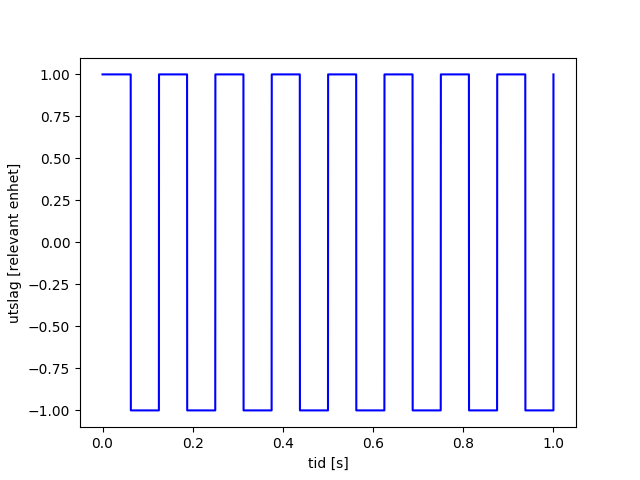
\includegraphics[width=12.6cm,height=9cm]{3Figur_21.png} \\
\caption{Firkantbølge med amplitude $1$ og frekvens $16$}
				\end{figure}
				\begin{figure}[H]
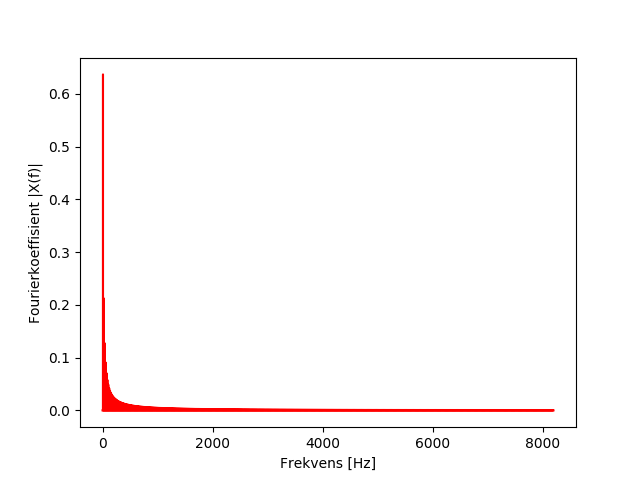
\includegraphics[width=12.6cm,height=9cm]{3Figur_22.png} \\
\caption{Fouriertransformasjon av sinusbølgen over}
				\end{figure}
\lstinputlisting{Oblig3_5_16.py}










		\paragraph{14)}
			\subparagraph{8.}
				\begin{flushleft}
Plotter funksjonen med variablene som er oppgitt i oppgaven, men bare den første førtiendedelen av bølgen.
				\end{flushleft}
				\begin{figure}[H]
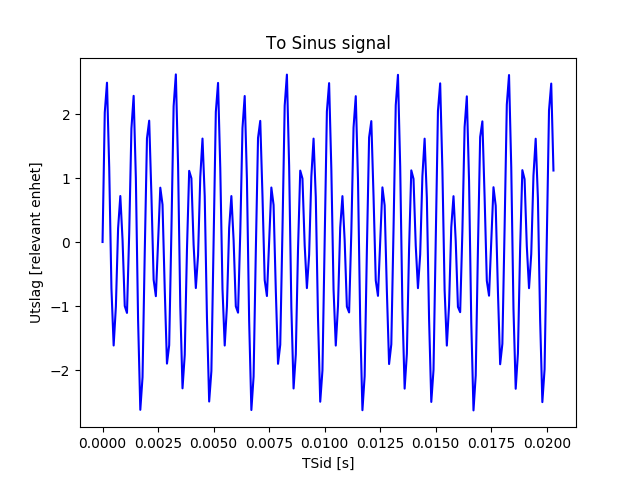
\includegraphics[width=12.6cm,height=9cm]{3Figur_23.png} \\
\caption{Plott av bølgen som skal analyseres}
				\end{figure}




				\begin{flushleft}
Deretter kjører jeg en vanlig FFT slik som tidligere gjort, og plotter resultatet, men bare halvparten av frekvensene for ikke å få speiling. Ser at vi får to topper ved $1000$ og $1600$ som er akkurat det vi forventet. Høyden blir også halvparten av amplituden til de to bølgene som sammen utgjør signalet vi skal analysere.
				\end{flushleft}
				\begin{figure}[H]
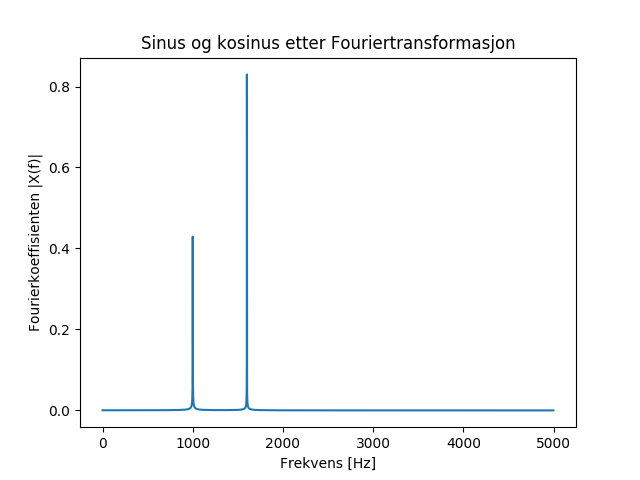
\includegraphics[width=12.6cm,height=9cm]{3Figur_24.png} \\
\caption{Frekvensbildet til signalet, funnet ved hjelp av FFT}
				\end{figure}






				\begin{flushleft}
Beregner den wavelettransformerte ved hjelp av en Morlet wavelet, fra $800 Hz$ til $2000 Hz$ logaritmisk fordelt, på den effektive måten beskrevet i boka. Setter først $K = 24$ og deretter $K = 200$. Ut ifra disse valgte K verdiene er det kanske greit å se at signalet har to frekvenser på ganske presist $1000$ og $1600$. I tillegg er disse frekvensene konstante gjennom hele tidsperioden.
				\end{flushleft}
				\begin{figure}[H]
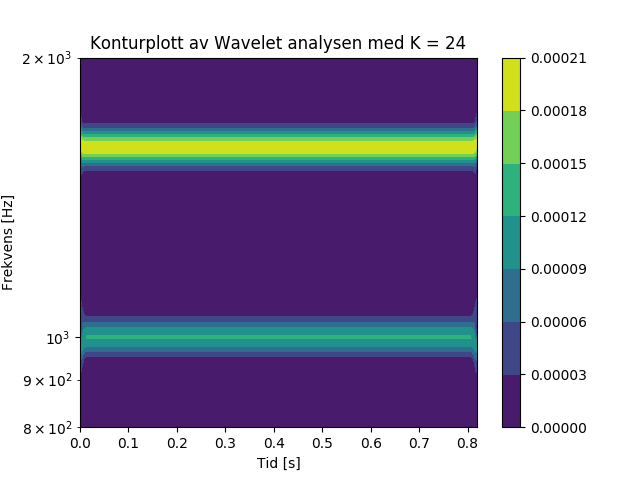
\includegraphics[width=12.6cm,height=9cm]{3Figur_25.png}
				\end{figure}
				\begin{figure}[H]
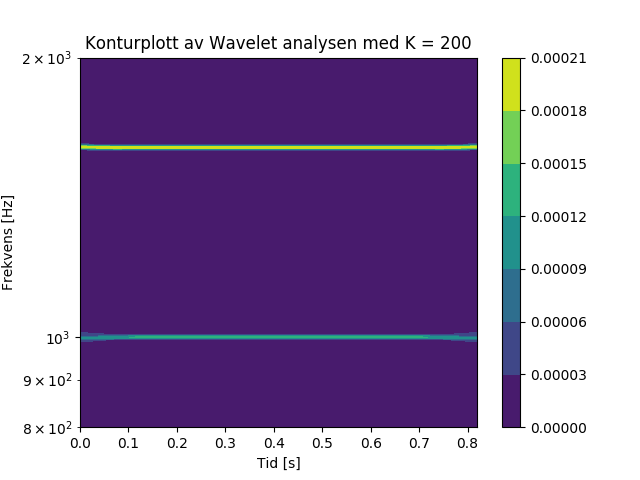
\includegraphics[width=12.6cm,height=9cm]{3Figur_26.png}
				\end{figure}








				\begin{flushleft}
Til lager jeg det nye signalet, med de samme konstantene fra tidligere, men lagt til fire nye, og på en annen form enn tidligere. Gjennomfører Fouriertransformasjonen og bruker samme funksjon jeg lagde tidligere til å gjøre en wavelettanalyse. Denne gangen analyserer jeg derimot frekvensene fra $800$ til $2000$, med $M$ antall frekvenssteg, der $M$ er gitt av utrykket på side $433$ i læreboka. Dette gjør jeg for $K$ verdiene lik $8$, $24$, $100$ og $200$. Til slutt plotter jeg alle de seks figurene. Signalet i tidsbildet blir veldig kult, dog noe hakkete av mangel på punkter når vi zoomer såpass mye inn, og i frekvensbildet blir det to topper slik som tidligere. Toppen ved $1000 Hz$ blir til forskjell fra tidligere mye bredere da. Fra wavelet transformasjonen får jeg to flekker, en ved frekvens lik $1000 Hz$ og tiden lik $0.15 s$, og den andre ved $1600 Hz$ og $0.5 s$. Unntaket er når jeg setter $K = 200$. Da får jeg bare en flekk, altså den nederste flekken til venstre forsvinner. Det at den ene flekken forsvinner kan komme av at den varer over såpass kort tid, noe vi ser fra plottet for $K = 8$, at den ikke får gitt nok bidrag til å bli med i analysen når den store $K$ verdien gjør at tidsoppløsningen blir dårlig.
				\end{flushleft}
				\begin{figure}[H]
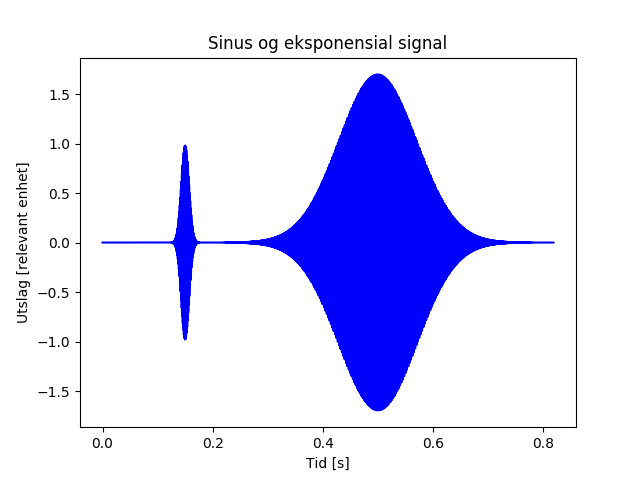
\includegraphics[width=12.6cm,height=9cm]{3Figur_27.png}
				\end{figure}
				\begin{figure}[H]
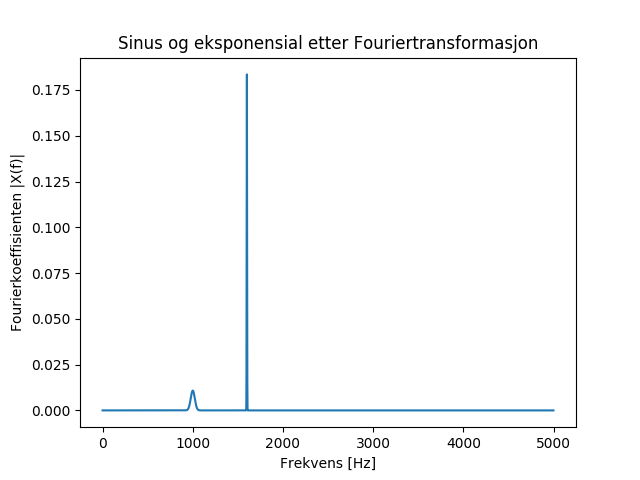
\includegraphics[width=12.6cm,height=9cm]{3Figur_28.png}
				\end{figure}
				\begin{figure}[H]
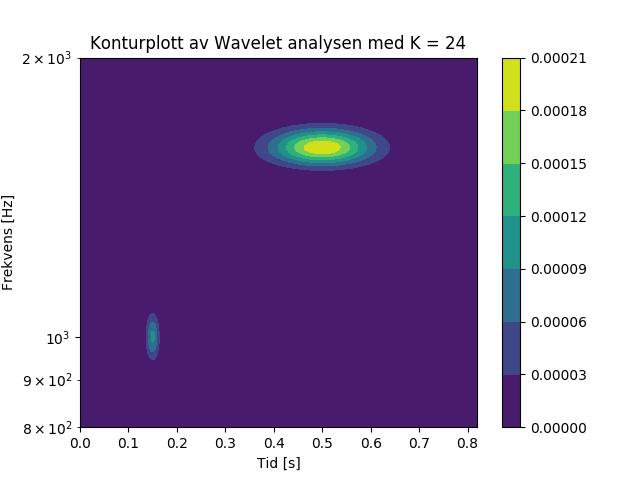
\includegraphics[width=12.6cm,height=9cm]{3Figur_29.png}
				\end{figure}
				\begin{figure}[H]
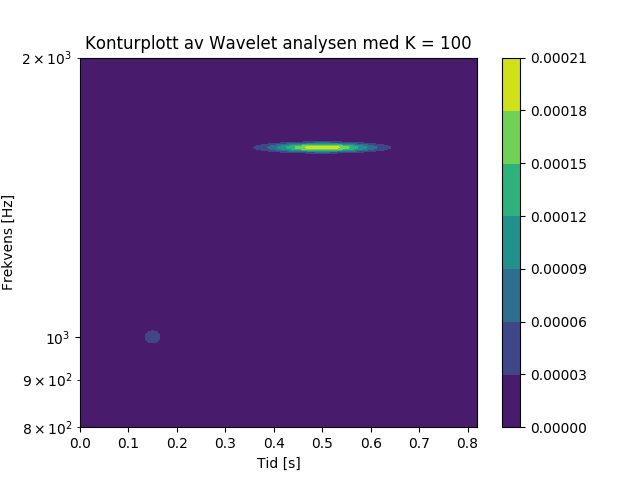
\includegraphics[width=12.6cm,height=9cm]{3Figur_30.png}
				\end{figure}
				\begin{figure}[H]
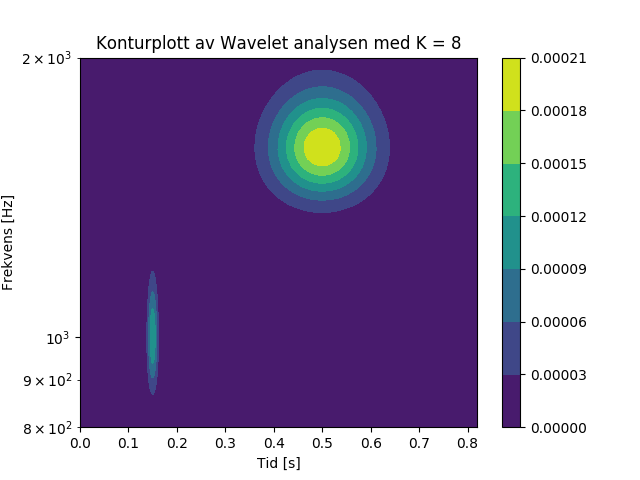
\includegraphics[width=12.6cm,height=9cm]{3Figur_31.png}
				\end{figure}
				\begin{figure}[H]
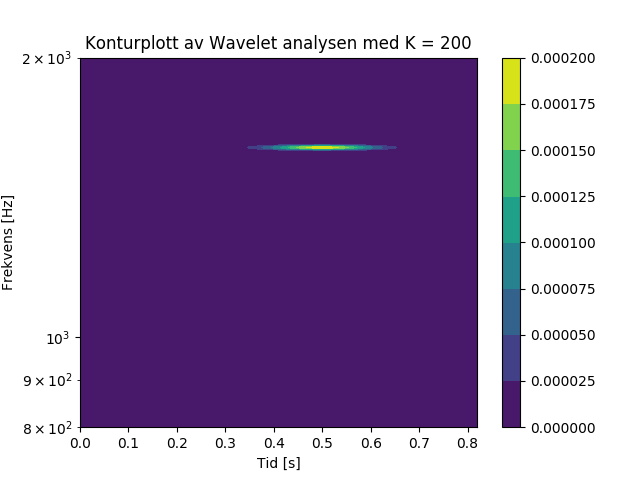
\includegraphics[width=12.6cm,height=9cm]{3Figur_32.png}
				\end{figure}
\lstinputlisting{Oblig3_14_8.py}
\end{document}